\frame
{
	\frametitle{RNA-seq Experiments}

	\vspace{-0.05cm}
	\begin{columns}[c]
	\column{0.48\textwidth} 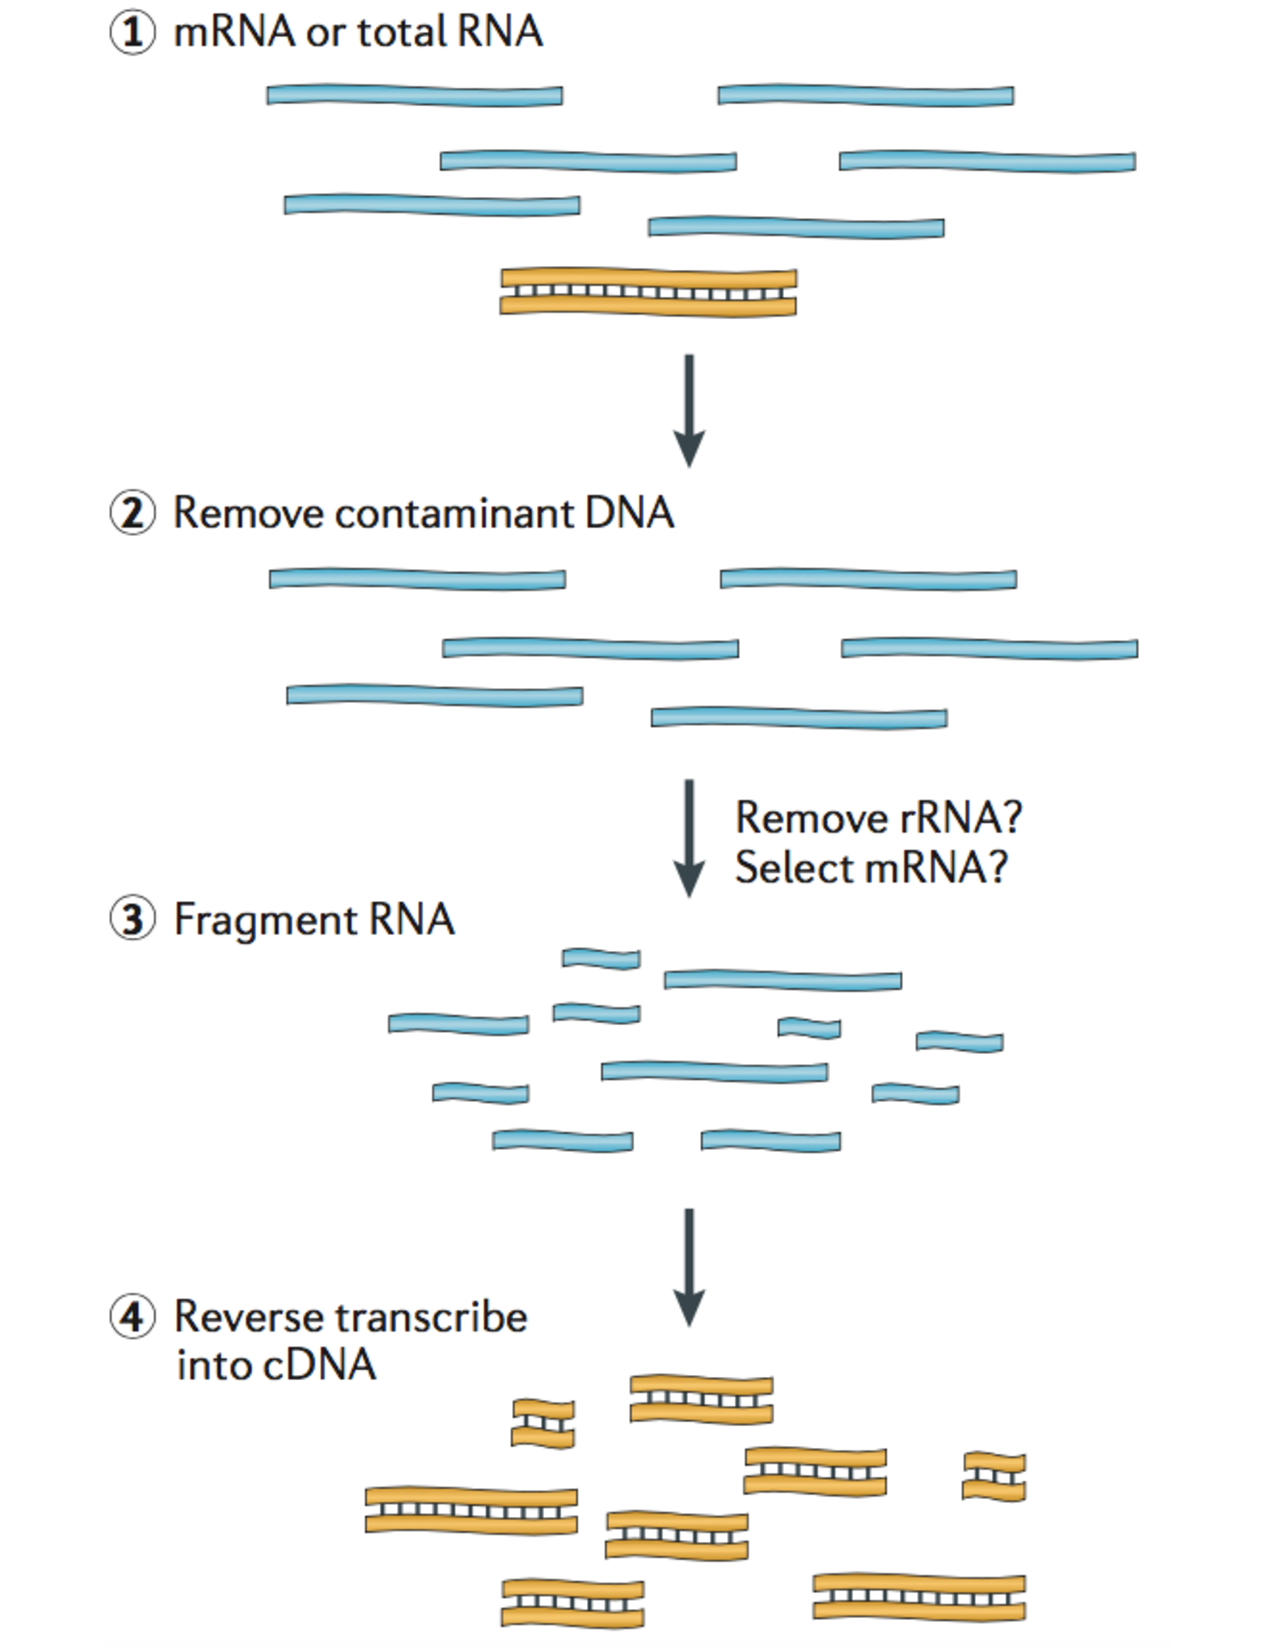
\includegraphics[width=\textwidth]{figures/seq1.pdf}
	\column{0.48\textwidth} 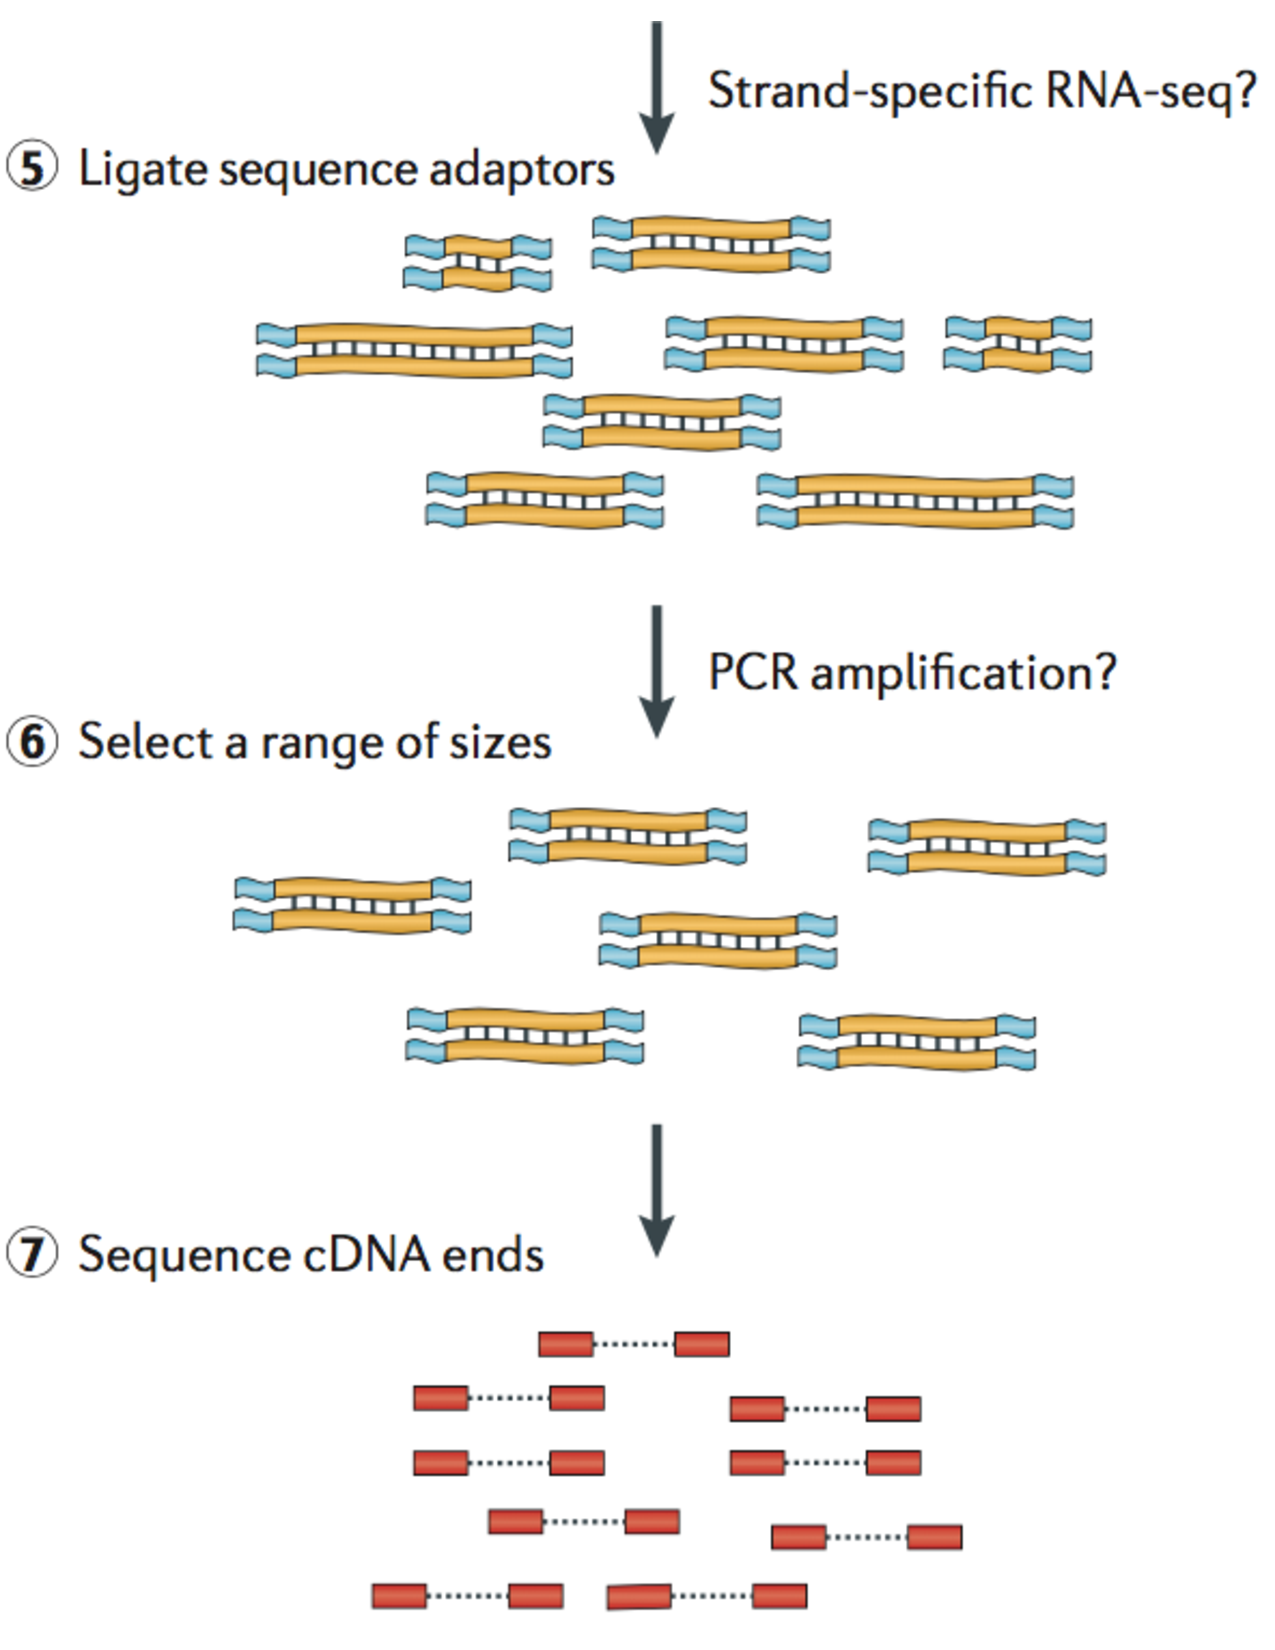
\includegraphics[width=\textwidth]{figures/seq2.pdf}
	\end{columns}

	\vspace{0.25cm}
	\onslide<2->{{\bf Transcriptome Assembly:} To determine the transcripts and their abundance from the (paired-end) reads.}
}

\frame
{
	\frametitle{Existing Softwares/Methods}
	\begin{itemize}
	\item {\bf Reference-based} methods:
		\vspace{0.05cm}
		\begin{itemize}
		\item Cufflinks~(Trapnell \emph{et al.}, 2010) \hspace{0.7cm}\onslide<2->{{\bf use overlap graph}}
		\vspace{-0.05cm}
		\[\left.\hspace{-0.98cm}\parbox{0.5\textwidth}{%
		\item Scripture~(Guttman \emph{et al.}, 2010)
		\vspace{0.05cm}
		\item IsoLasso~(Li \emph{et al.}, 2011)
		\vspace{0.05cm}
		\item SLIDE~(Li \emph{et al.}, 2011)
		\vspace{0.05cm}
		\item CLIIQ~(Lin \emph{et al.}, 2012)
		\vspace{0.05cm}
		\item CEM~(Li \emph{et al.}, 2012)
		\vspace{0.05cm}
		\item MITIE~(Behr \emph{et al.}, 2013)
		\vspace{0.05cm}
		\item Traph~(Tomescu \emph{et al.}, 2013)
		\vspace{0.05cm}
		\item StringTie~(Pertea \emph{et al.}, 2015)}
		\onslide<2->{\right\} \textsf{\bf use splice graph}}\]
		\vspace{-0.2cm}
		\item {\bf ...}
		\end{itemize}
	\vspace{0.2cm}
	\item {\bf\emph{De novo}} methods:
		\vspace{0.05cm}
		\begin{itemize}
		\item Trans-ABySS~(Robertson \emph{et al.}, 2010)
		\vspace{0.05cm}
		\item Trinity~(Grabherr \emph{et al.}, 2011)
		\vspace{0.05cm}
		\item Oases~(Schulz \emph{et al.}, 2012)
		\vspace{0.05cm}
		\item {\bf ...}
		\end{itemize}
	\end{itemize}
}

\frame
{
	\frametitle{Splice Graph}
	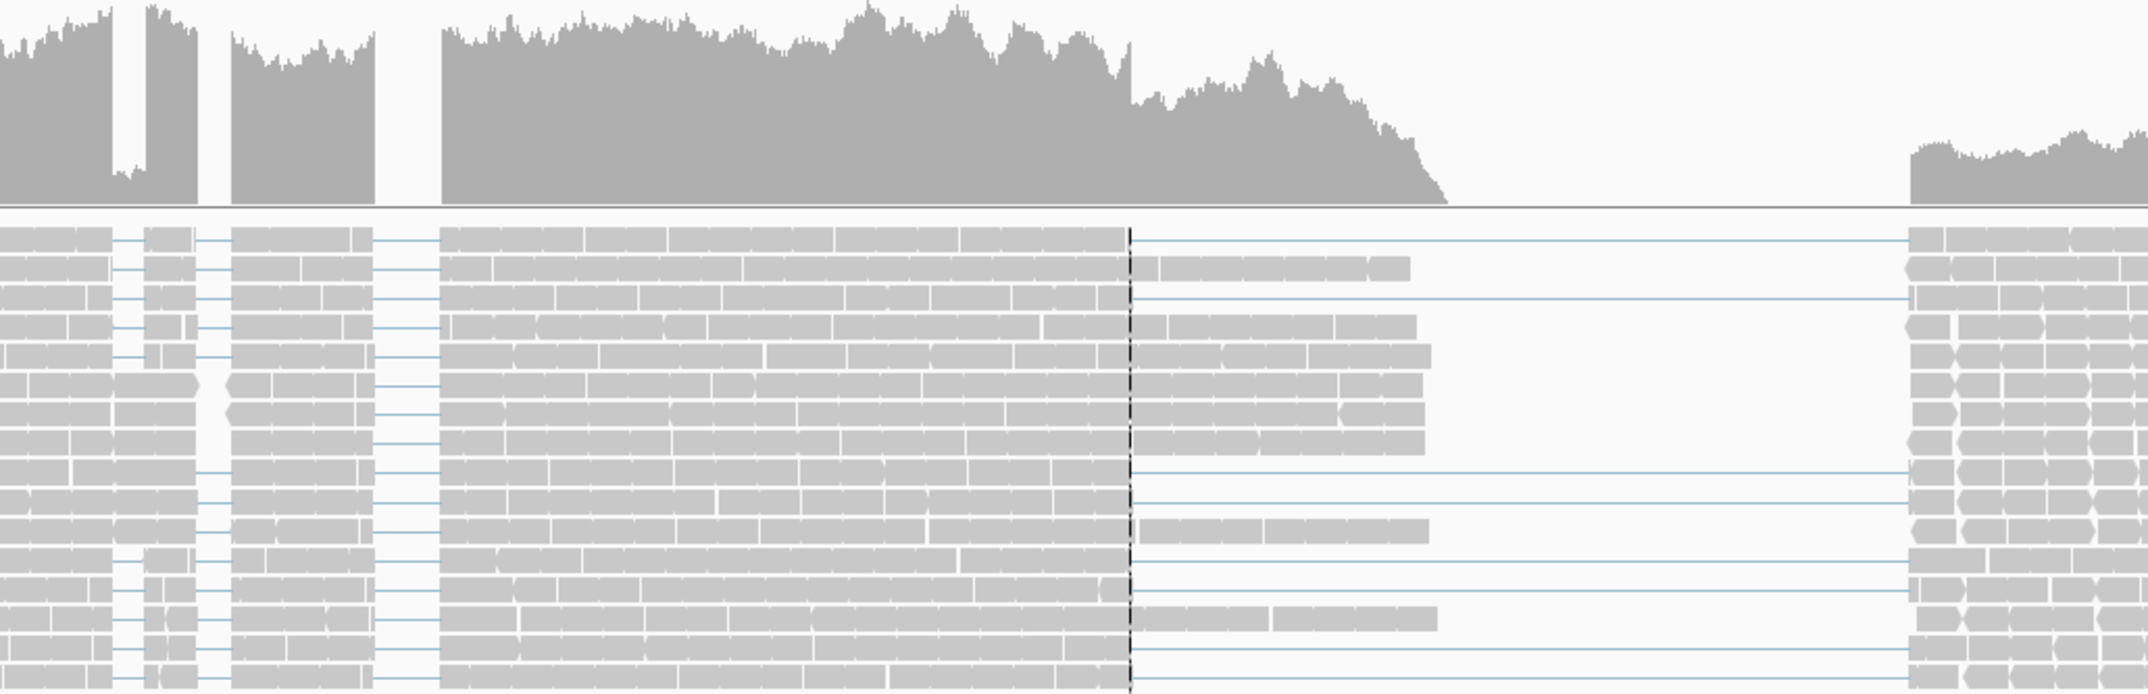
\includegraphics[width=\textwidth]{figures/reference.pdf}
	\vspace{0.2cm}
	\begin{center}

\begin{tikzpicture}[font=\small,overlay,
mycirclex/.style={draw, circle, minimum size=1.0em, inner sep = 0.2mm}, 
mydiamond/.style={draw, diamond, minimum size=0.78em, inner sep = 0mm}, 
myrectang/.style={draw, rectangle, minimum size=0.60em, inner sep = 0mm}, 
>=stealth]

\begin{scope}[xshift = -6cm, yshift=3.5cm]
\path<2-> node[blue] at (0.9cm, 0) {$1$};
\path<2-> node[blue] at (1.25cm, 0) {$2$};
\path<2-> node[blue] at (1.47cm,0) {$3$};
\path<2-> node[blue] at (2.1cm, 0) {$4$};
\path<2-> node[blue] at (4.5cm, 0) {$5$};
\path<2-> node[blue] at (7.0cm, 0) {$6$};
\path<2-> node[blue] at(10.8cm, 0) {$7$};
\end{scope}


\end{tikzpicture}
\end{center}

	\vspace{-0.4cm}
	\begin{center}

\begin{tikzpicture}[font=\small,overlay,
mycirclex/.style={draw, circle, minimum size=1.0em, inner sep = 0.2mm}, 
mydiamond/.style={draw, diamond, minimum size=0.78em, inner sep = 0mm}, 
myrectang/.style={draw, rectangle, minimum size=0.60em, inner sep = 0mm}, 
>=stealth]

\definecolor{mygreen}{rgb}{0, 0.7, 0}
\definecolor{myyellow}{rgb}{0.8, 0.6, 0}

\def\colx{black}
\def\cola{red} 
\def\colb{blue}
\def\colc{violet}
\def\cold{cyan} 
\def\cole{myyellow}
\def\colf{brown}


\def\len{2.0cm}

% G1
\begin{scope}[local bounding box=bbox, xshift=-6.0cm]
\path<1-> node[mycirclex] (v1) at (1.0 * \len, 0) {$s$};
\path<1-> node[mycirclex] (v2) at (2.0 * \len, 0) {$a$};
\path<1-> node[mycirclex] (v3) at (3.0 * \len, 0) {$b$};
\path<1-> node[mycirclex] (v4) at (4.0 * \len, 0) {$c$};
\path<1-> node[mycirclex] (v5) at (5.0 * \len, 0) {$t$};

\path<1-> [draw, \colx, ->, line width=0.04cm] (v1) -- (v2);
\path<1-> [draw, \colx, ->, line width=0.04cm] (v2) -- (v3);
\path<1-> [draw, \colx, ->, line width=0.04cm] (v3) -- (v4);
\path<1-> [draw, \colx, ->, line width=0.04cm] (v4) -- (v5);

\path<1-> [draw, \colx, ->, line width=0.04cm, bend left = 40] (v1) to (v3);
\path<1-> [draw, \colx, ->, line width=0.04cm, bend left = 40] (v3) to (v5);
\path<1-> [draw, \colx, ->, line width=0.04cm, bend left = 40] (v2) to (v4);

\path<1-> node at (1.5 * \len, 0.18cm) {$e_1(8)$};
\path<1-> node at (2.5 * \len, 0.18cm) {$e_2(2)$};
\path<1-> node at (3.5 * \len, 0.18cm) {$e_3(4)$};
\path<1-> node at (4.5 * \len, 0.18cm) {$e_4(10)$};

\path<1-> node at (2.0 * \len, 1.0cm) {$e_5(5)$};
\path<1-> node at (3.0 * \len, 1.0cm) {$e_6(6)$};
\path<1-> node at (4.0 * \len, 1.0cm) {$e_7(3)$};

\end{scope}
%\path<1-> [draw, rounded corners] ($(bbox.south west) - (0.00cm, 0.25cm)$) rectangle ($(bbox.north east) + (0.1cm, 0)$);
%\node at ($(bbox.south) - (0.00cm, 0.2cm)$) [label=below:{$G_2 - G_1 = \{c\}$}]{};


\end{tikzpicture}
\end{center}

	\vspace{0.2cm}
	\begin{itemize}
	\item<3-> {\bf Nodes:} continuous regions not seperated by spliced reads
	\item<3-> {\bf Edges:} adjacent regions or connected by spliced reads
	\item<4-> {\bf Weight of nodes:} estimated from the average coverage
	\item<4-> {\bf Weight of edges:} estimated from number of spanning reads
	\end{itemize}
}

\frame
{
	\frametitle{Optimization Problem}

	\begin{itemize}
	\item {\bf Input:} Directed acyclic graph~(DAG) $G=(V,E)$ with a single source $s$ and a single sink $t$;
		weight $w(e)$ for $e\in E$.

	\vspace{0.2cm}

	\item {\bf Output:} A set of $s$-$t$ paths $\mathcal{P}$ and abundance $a(P)$ for $P\in\mathcal{P}$, such that
		\begin{enumerate}
		\vspace{0.1cm}
		\item each $e\in E$ is covered by at least one path $P\in\mathcal{P}$, and that
		\vspace{0.1cm}
		\item $|\mathcal{P}|$ is as small as possible, and that
		\vspace{0.1cm}
		\item $\sum_{e\in E} \|w(e) - \sum_{P:e\in P} a(P)\|$ is as small as possible.
		\end{enumerate}
	\end{itemize}

	\vspace{1.0cm}
	\begin{center}

\begin{tikzpicture}[font=\small,overlay,
mycirclex/.style={draw, circle, minimum size=1.0em, inner sep = 0.2mm}, 
mydiamond/.style={draw, diamond, minimum size=0.78em, inner sep = 0mm}, 
myrectang/.style={draw, rectangle, minimum size=0.60em, inner sep = 0mm}, 
>=stealth]

\definecolor{mygreen}{rgb}{0, 0.7, 0}
\definecolor{myyellow}{rgb}{0.8, 0.6, 0}

\def\colx{black}
\def\cola{red} 
\def\colb{blue}
\def\colc{violet}
\def\cold{cyan} 
\def\cole{myyellow}
\def\colf{brown}


\def\len{3.0cm}

% G1
\begin{scope}[local bounding box=bbox, xshift=-8.0cm]
\path<1-> node[mycirclex] (v1) at (1.0 * \len, 0) {$s$};
\path<1-> node[mycirclex] (v2) at (2.0 * \len, 0) {$a$};
\path<1-> node[mycirclex] (v3) at (3.0 * \len, 0) {$b$};
\path<1-> node[mycirclex] (v4) at (4.0 * \len, 0) {$t$};

\path<1-> [draw, \colc, ->, line width=0.04cm] (v1) -- (v2);
\path<1-> [draw, \colc, ->, line width=0.10cm, bend left = 40] (v2) to (v3);
\path<1-> [draw, \colc, ->, line width=0.10cm, bend left = 40] (v3) to (v4);

\path<1-> [draw, \colb, ->, line width=0.04cm] (v2) -- (v3);
\path<1-> [draw, \colb, ->, line width=0.10cm, bend left = 40] (v1) to (v2);
\path<1-> [draw, \colb, ->, line width=0.04cm, bend left = 40] (v3) to (v4);

\path<1-> [draw, \cola, ->, line width=0.04cm] (v3) -- (v4);
\path<1-> [draw, \cola, ->, line width=0.04cm, bend left = 40] (v1) to (v2);
\path<1-> [draw, \cola, ->, line width=0.04cm, bend left = 40] (v2) to (v3);


%\path<1-> [draw, \colx, ->, line width=0.02cm] (v1) -- (v2);
%\path<1-> [draw, \colx, ->, line width=0.02cm] (v2) -- (v3);
%\path<1-> [draw, \colx, ->, line width=0.02cm] (v3) -- (v4);
%
%\path<1-> [draw, \colx, ->, line width=0.02cm, bend left = 40] (v1) to (v2);
%\path<1-> [draw, \colx, ->, line width=0.02cm, bend left = 40] (v2) to (v3);
%\path<1-> [draw, \colx, ->, line width=0.02cm, bend left = 40] (v3) to (v4);

\path<1-> node at (1.5 * \len, 0.18cm) {$e_2(4)$};
\path<1-> node at (2.5 * \len, 0.18cm) {$e_4(3)$};
\path<1-> node at (3.5 * \len, 0.18cm) {$e_6(2)$};

\path<1-> node at (1.5 * \len, 0.85cm) {$e_1(5)$};
\path<1-> node at (2.5 * \len, 0.85cm) {$e_3(6)$};
\path<1-> node at (3.5 * \len, 0.85cm) {$e_5(7)$};

\end{scope}
%\path<1-> [draw, rounded corners] ($(bbox.south west) - (0.00cm, 0.25cm)$) rectangle ($(bbox.north east) + (0.1cm, 0)$);
%\node at ($(bbox.south) - (0.00cm, 0.2cm)$) [label=below:{$G_2 - G_1 = \{c\}$}]{};


\end{tikzpicture}
\end{center}

	\vspace{1.0cm}
}

\frame
{
	\frametitle{Minimize the Number of Paths}
	{\bf Problem:} Given DAG $G=(V,E)$ with source $s$ and sink $t$, 
		to compute minimum number of paths that can cover all edges.

	\vspace{0.4cm}

	\begin{center}

\begin{tikzpicture}[font=\small,overlay,
mycirclex/.style={draw, circle, minimum size=1.0em, inner sep = 0.2mm}, 
mydiamond/.style={draw, diamond, minimum size=0.78em, inner sep = 0mm}, 
myrectang/.style={draw, rectangle, minimum size=0.60em, inner sep = 0mm}, 
>=stealth]

\definecolor{mygreen}{rgb}{0, 0.7, 0}
\definecolor{myyellow}{rgb}{0.8, 0.6, 0}

\def\colx{black}
\def\cola{red} 
\def\colb{blue}
\def\colc{violet}
\def\cold{cyan} 
\def\cole{myyellow}
\def\colf{brown}


\def\len{1.8cm}

% G1
\begin{scope}[local bounding box=bbox, xshift=-6.4cm]
\path<1-> node[mycirclex] (v1) at (1.0 * \len, 0) {$s$};
\path<1-> node[mycirclex] (v2) at (2.0 * \len, 0) {$a$};
\path<1-> node[mycirclex] (v3) at (3.0 * \len, 0) {$b$};
\path<1-> node[mycirclex] (v4) at (4.0 * \len, 0) {$c$};
\path<1-> node[mycirclex] (v5) at (5.0 * \len, 0) {$d$};

\path<1-> [draw, \colx, ->, line width=0.04cm] (v1) -- (v2);
\path<1-> [draw, \colx, ->, line width=0.04cm] (v2) -- (v3);
\path<1-> [draw, \colx, ->, line width=0.04cm] (v3) -- (v4);
\path<1-> [draw, \colx, ->, line width=0.04cm] (v4) -- (v5);

\path<1-> [draw, \colx, ->, line width=0.04cm, bend left = 40] (v1) to (v3);
\path<1-> [draw, \colx, ->, line width=0.04cm, bend left = 27] (v2) to (v5);
\path<1-> [draw, \colx, ->, line width=0.04cm, bend left =-40] (v2) to (v4);

\path<1-> node at (1.5 * \len, 0.18cm) {$e_1$};
\path<1-> node at (2.5 * \len, 0.18cm) {$e_2$};
\path<1-> node at (3.5 * \len, 0.18cm) {$e_3$};
\path<1-> node at (4.5 * \len, 0.18cm) {$e_4$};

\path<1-> node at (2.0 * \len, 0.9cm) {$e_5$};
\path<1-> node at (3.0 * \len,-0.6cm) {$e_6$};
\path<1-> node at (3.5 * \len, 0.9cm) {$e_7$};

\end{scope}
%\path<1-> [draw, rounded corners] ($(bbox.south west) - (0.00cm, 0.25cm)$) rectangle ($(bbox.north east) + (0.1cm, 0)$);
%\node at ($(bbox.south) - (0.00cm, 0.2cm)$) [label=below:{$G_2 - G_1 = \{c\}$}]{};


\end{tikzpicture}
\end{center}


	\vspace{0.6cm}

	\onslide<2->{{\bf Polynomial-time Algorithm:}}
	\vspace{-0.2cm}
	\begin{center}

\begin{tikzpicture}[font=\small,overlay,
mycirclex/.style={draw, circle, minimum size=1.0em, inner sep = 0.2mm}, 
mydiamond/.style={draw, diamond, minimum size=0.78em, inner sep = 0mm}, 
myrectang/.style={draw, rectangle, minimum size=0.60em, inner sep = 0mm}, 
>=stealth]

\definecolor{mygreen}{rgb}{0, 0.7, 0}
\definecolor{myyellow}{rgb}{0.8, 0.6, 0}

\def\colx{black}
\def\cola{red} 
\def\colb{blue}
\def\colc{violet}
\def\cold{cyan} 
\def\cole{myyellow}
\def\colf{brown}


\def\len{1.2cm}

% G1
\begin{scope}[local bounding box=bbox, xshift=-5.5cm]
\path<2-> node[mycirclex] (x1) at (1.0 * \len, 0.0) {$e_1$};
\path<2-> node[mycirclex] (x2) at (2.0 * \len, 0.0) {$e_2$};
\path<2-> node[mycirclex] (x3) at (3.0 * \len, 0.0) {$e_3$};
\path<2-> node[mycirclex] (x4) at (4.0 * \len, 0.0) {$e_4$};
\path<2-> node[mycirclex] (x5) at (5.0 * \len, 0.0) {$e_5$};
\path<2-> node[mycirclex] (x6) at (6.0 * \len, 0.0) {$e_6$};
\path<2-> node[mycirclex] (x7) at (7.0 * \len, 0.0) {$e_7$};

\path<2-> node[mycirclex] (y1) at (1.0 * \len, -2.0) {$e_1$};
\path<2-> node[mycirclex] (y2) at (2.0 * \len, -2.0) {$e_2$};
\path<2-> node[mycirclex] (y3) at (3.0 * \len, -2.0) {$e_3$};
\path<2-> node[mycirclex] (y4) at (4.0 * \len, -2.0) {$e_4$};
\path<2-> node[mycirclex] (y5) at (5.0 * \len, -2.0) {$e_5$};
\path<2-> node[mycirclex] (y6) at (6.0 * \len, -2.0) {$e_6$};
\path<2-> node[mycirclex] (y7) at (7.0 * \len, -2.0) {$e_7$};

\path<3-> [draw, \cola, line width=0.08cm] (x1) -- (y2);
\path<3-> [draw, \cola, line width=0.08cm] (x2) -- (y3);
\path<3-> [draw, \cola, line width=0.08cm] (x5) -- (y4);

\path<2-> [draw, \colx, line width=0.03cm] (x1) -- (y2);
\path<2-> [draw, \colx, line width=0.03cm] (x1) -- (y3);
\path<2-> [draw, \colx, line width=0.03cm] (x1) -- (y4);
\path<2-> [draw, \colx, line width=0.03cm] (x1) -- (y6);
\path<2-> [draw, \colx, line width=0.03cm] (x1) -- (y7);
\path<2-> [draw, \colx, line width=0.03cm] (x2) -- (y3);
\path<2-> [draw, \colx, line width=0.03cm] (x2) -- (y4);
\path<2-> [draw, \colx, line width=0.03cm] (x3) -- (y4);
\path<2-> [draw, \colx, line width=0.03cm] (x5) -- (y3);
\path<2-> [draw, \colx, line width=0.03cm] (x5) -- (y4);
\path<2-> [draw, \colx, line width=0.03cm] (x6) -- (y4);

\end{scope}
%\path<2-> [draw, rounded corners] ($(bbox.south west) - (0.00cm, 0.25cm)$) rectangle ($(bbox.north east) + (0.1cm, 0)$);
%\node at ($(bbox.south) - (0.00cm, 0.2cm)$) [label=below:{$G_2 - G_1 = \{c\}$}]{};


\end{tikzpicture}
\end{center}


	\vspace{2.0cm}
	\onslide<4->{{\bf Dilworth's Theorem:} $|\mathcal{P}| = |E| - M$.}
	
	\vspace{0.2cm}
	\onslide<5->{{\bf Existing Software:} Cufflinks~(Trapnell \emph{et al.}, 2010)}
}

\frame
{
	\frametitle{Minimize Abundance Error}
	{\bf Problem:} Given DAG $G=(V,E)$ with source $s$, sink $t$, and weight $w(e)$
	for $e\in E$, to compute a set of $s$-$t$ paths $\mathcal{P}$ so that all edges
	are covered and that $\sum_{e\in E} |w(e) - \sum_{P:e\in P} a(P)|$ is minimized.

	\vspace{0.2cm}
	\onslide<2->{{\bf Fact:} There exists a set of paths satisfying $x(e) = \sum_{P\in\mathcal{P}:e\in P} a(P)$ 
		for all $e\in E$ if and only if $x(e)$ forms a flow of $G$.}

	\vspace{0.2cm}
	\onslide<3->{{\bf Reformulation:} To compute $x(e)$ for $e\in E$ such that $x(e)$ forms a flow
		and that $\sum_{e\in E} |w(e) - x(e)|$ is minimized.}

	\vspace{0.2cm}
	\onslide<4->{{\bf Polynomial-time Algorithm}~(using LP):
	\begin{displaymath}
	\displaystyle
	\begin{array}{rl}
	\min & \sum_{e\in E} |w(e) - x(e)| \\
	\textrm{s.t.} & \left\{
		\begin{array}{ll}
			\sum_{e=(u,v)\in E} x(e) = \sum_{e=(v,w)\in E} x(e), \forall v \in V\\
			x(e) \ge 0, \forall e\in E
		\end{array}
		\right.
	\end{array}
	\end{displaymath}}

	\onslide<5->{Based on $x(e)$, {\bf greedy algorithm} can be used to retrieve $\mathcal{P}$
	with at most $|E| - |V| + 2$ paths.}

	\vspace{0.2cm}
	\onslide<6->{{\bf Existing Software:} Traph~(Tomescu \emph{et al.}, 2013)}
}

\frame
{
	\frametitle{Minimize Abundance Error with $k$ Paths}
	{\bf Problem:} Given DAG $G=(V,E)$ with source $s$, sink $t$, weight $w(e)$ for $e\in E$,
		to compute a set of at most $k$ $s$-$t$ paths $\mathcal{P}$ such that
			$\sum_{e\in E} \| w(e) - \sum_{P:e\in P} a(P)\|$ is minimized.

	\vspace{0.3cm}
	\onslide<2->{{\bf Maximum $k$-Splittable Flow Problem:} Given DAG $G=(V,E)$ with source
	$s$, sink $t$, weight $w(e)$ for $e\in E$, to compute a set of at most $k$
	$s$-$t$ paths $\mathcal{P}$ satisfying $\sum_{P:e\in P} a(P)\le w(e), \forall e\in E$~(capacity constraints) such that 
	$\sum_{P\in\mathcal{P}} a(P)$ is maximized.}

	\vspace{0.2cm}
	\begin{enumerate}
	\item<3-> {M$k$SF is {\bf NP}-hard for $2\le k < |E| - |V| + 2$.}
	\vspace{0.1cm}
	\item<4-> 1.5-approximation algorithm for $k=2$ and $k=3$.
	\vspace{0.1cm}
	\item<5-> 2-approximation algorithm for $4\le k < |E| - |V| + 2$.
	\vspace{0.1cm}
	\item<6-> Polynomial-time algorithm for $G$ with constant treewidth.
	\end{enumerate}
}

\frame
{
	\frametitle{Regularization Methods}

	{\bf Optimization Formulation:}
	\begin{displaymath}
	\min  \sum_{e\in E} \|w(e) - \sum_{P:e\in P} a(P)\| + \lambda \sum_{P\in\mathcal{P}} \|a(P)\|^q
	\end{displaymath}

	\vspace{0.2cm}
	\onslide<2->{
	\begin{enumerate}
	\item Initialize $\mathcal{P}$ as all possible paths~(exponential size).
	\item Parameter $\lambda$ needs to be trained.
	\item Use continuous optimization techniques~(Lasso, Newton–Raphson, etc) to compute a local optimal solution.
	\end{enumerate}}

	\vspace{0.2cm}
	\onslide<3->{{\bf Existing Softwares:} IsoLasso~(Li \emph{et al.}, 2011), SLIDE~(Li \emph{et al.}, 2011),
		CEM~(Li \emph{et al.}, 2012), MITIE~(Behr \emph{et al.}, 2013)}
}

\frame
{
	\frametitle{Heuristic---Greedy Algorithm}

	{\bf Algorithm:} Iteratively compute the path with maximum bottleneck weight, and then update the graph.
	\vspace{0.7cm}
	\begin{center}

\begin{tikzpicture}[font=\small,overlay,
mycirclex/.style={draw, circle, minimum size=1.0em, inner sep = 0.2mm}, 
mydiamond/.style={draw, diamond, minimum size=0.78em, inner sep = 0mm}, 
myrectang/.style={draw, rectangle, minimum size=0.60em, inner sep = 0mm}, 
>=stealth]

\definecolor{mygreen}{rgb}{0, 0.7, 0}
\definecolor{myyellow}{rgb}{0.8, 0.6, 0}

\def\colx{black}
\def\cola{red} 
\def\colb{blue}
\def\colc{violet}
\def\cold{cyan} 
\def\cole{myyellow}
\def\colf{brown}


\def\len{1.5cm}

% G1
\begin{scope}[local bounding box=bbox, xshift=-6cm]
\path<2-> node[mycirclex] (v1) at (1.0 * \len, 0) {$s$};
\path<2-> node[mycirclex] (v2) at (2.0 * \len, 0) {$a$};
\path<2-> node[mycirclex] (v3) at (3.0 * \len, 0) {$b$};
\path<2-> node[mycirclex] (v4) at (4.0 * \len, 0) {$c$};
\path<2-> node[mycirclex] (v5) at (5.0 * \len, 0) {$d$};
\path<2-> node[mycirclex] (v6) at (6.0 * \len, 0) {$t$};

\path<3-> [draw, \cola, ->, line width=0.09cm, bend left = 40] (v1) to (v3);
\path<3-> [draw, \cola, ->, line width=0.09cm] (v3) -- (v4);
\path<3-> [draw, \cola, ->, line width=0.09cm] (v4) -- (v5);
\path<3-> [draw, \cola, ->, line width=0.09cm] (v5) -- (v6);

\path<2-> [draw, \colx, ->, line width=0.04cm] (v1) -- (v2);
\path<2-> [draw, \colx, ->, line width=0.04cm] (v2) -- (v3);
\path<2-> [draw, \colx, ->, line width=0.04cm] (v3) -- (v4);
\path<2-> [draw, \colx, ->, line width=0.04cm] (v4) -- (v5);
\path<2-> [draw, \colx, ->, line width=0.04cm] (v5) -- (v6);

\path<2-> [draw, \colx, ->, line width=0.04cm, bend left = 40] (v1) to (v3);
\path<2-> [draw, \colx, ->, line width=0.04cm, bend left = 40] (v3) to (v5);
\path<2-> [draw, \colx, ->, line width=0.04cm, bend left =-27] (v2) to (v5);
\path<2-> [draw, \colx, ->, line width=0.04cm, bend left =-40] (v4) to (v6);

\path<2-> node at (1.5 * \len, 0.2cm) {$4$};
\path<2-> node at (2.5 * \len, 0.2cm) {$1$};
\path<2-> node at (3.5 * \len, 0.2cm) {$5$};
\path<2-> node at (4.5 * \len, 0.2cm) {$4$};
\path<2-> node at (5.5 * \len, 0.2cm) {$9$};

\path<2-> node at (2.0 * \len, 0.85cm) {$6$};
\path<2-> node at (4.0 * \len, 0.85cm) {$2$};
\path<2-> node at (5.0 * \len,-0.85cm) {$1$};
\path<2-> node at (3.5 * \len,-0.85cm) {$3$};

\path<4-> [draw, \colx, ->, line width=0.1cm] (3.5 * \len, -1.2cm) -- (3.5 * \len, -1.8cm);

\end{scope}

%\path<2-> [draw, rounded corners] ($(bbox.south west) - (0.00cm, 0.25cm)$) rectangle ($(bbox.north east) + (0.1cm, 0)$);
%\node at ($(bbox.south) - (0.00cm, 0.2cm)$) [label=below:{$G_2 - G_1 = \{c\}$}]{};


% G2
\begin{scope}[local bounding box=bbox, xshift=-6cm, yshift = -2.6cm]
\path<4-> node[mycirclex] (v1) at (1.0 * \len, 0) {$s$};
\path<4-> node[mycirclex] (v2) at (2.0 * \len, 0) {$a$};
\path<4-> node[mycirclex] (v3) at (3.0 * \len, 0) {$b$};
\path<4-> node[mycirclex] (v4) at (4.0 * \len, 0) {$c$};
\path<4-> node[mycirclex] (v5) at (5.0 * \len, 0) {$d$};
\path<4-> node[mycirclex] (v6) at (6.0 * \len, 0) {$t$};

\path<4-> [draw, \colx, ->, line width=0.04cm] (v1) -- (v2);
\path<4-> [draw, \colx, ->, line width=0.04cm] (v2) -- (v3);
\path<4-> [draw, \colx, ->, line width=0.04cm] (v3) -- (v4);
\path<4-> [draw, \colx, ->, line width=0.04cm] (v5) -- (v6);

\path<4-> [draw, \colx, ->, line width=0.04cm, bend left = 40] (v1) to (v3);
\path<4-> [draw, \colx, ->, line width=0.04cm, bend left = 40] (v3) to (v5);
\path<4-> [draw, \colx, ->, line width=0.04cm, bend left =-27] (v2) to (v5);
\path<4-> [draw, \colx, ->, line width=0.04cm, bend left =-40] (v4) to (v6);

\path<4-> node at (1.5 * \len, 0.2cm) {$4$};
\path<4-> node at (2.5 * \len, 0.2cm) {$1$};
\path<4-> node at (3.5 * \len, 0.2cm) {$1$};
\path<4-> node at (5.5 * \len, 0.2cm) {$5$};

\path<4-> node at (2.0 * \len, 0.85cm) {$2$};
\path<4-> node at (4.0 * \len, 0.85cm) {$2$};
\path<4-> node at (5.0 * \len,-0.85cm) {$1$};
\path<4-> node at (3.5 * \len,-0.85cm) {$3$};
\end{scope}


\end{tikzpicture}
\end{center}

	\vspace{3.5cm}
	\onslide<6->{{\bf Existing Softwares:} Traph~(Tomescu \emph{et al.}, 2013), StringTie~(Pertea \emph{et al.}, 2015)}
}
